\section{Durchführung}
\label{sec:Durchführung}
\subsection{Aufabu}
Zur Messung der Kennlinie wird der Aufbau genutzt der in Abbildung \ref{fig:aufbaukennlinie} gezeugt wird.
\begin{figure}
    \centering
    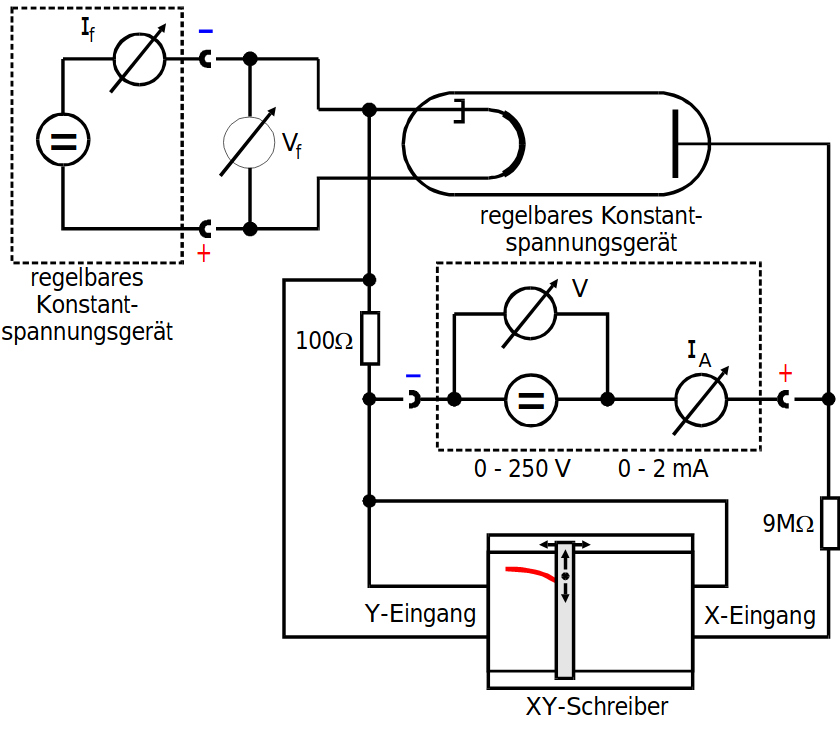
\includegraphics[width=0.7\textwidth]{content/data/aufbau_kennlinie.png}
    \caption{Der Aufbau welcher zur Messung der Kennlinie genutzt wird. Abbildung entnommen aus \cite[10]{anleitung}.}
    \label{fig:aufbaukennlinie}
\end{figure}
Der in der Abbildung zu sehende XY-Schreiber war leider nicht vorhabnden, deswegen wurden die Messwerte direkt vom Messgerät abgelesen.
Im oberen Teil der abbildung ist die Hochvakuum-Diode zu sehen.
An diese Wird ein ein Konstantspannungsgerät, welches links im Bild zu sehen ist, angeschlossen.
Mit diesem wird ein Heizstrom $I_\text{f}$ erzeugt, der zwischen $2-2.5 \SI{}{\A}$ liegt, sodass der Heizdraht nicht kaputt geht.
Zudem wird an der Diode eine weitere Spanungsquelle angebracht.
Diese erzeugt eine Beschleunigungsspannung zwischen Anode und Kathode.
Die Beschleuningungsspannung bewegt sich dabei von $0-250 \SI{}{\V}$.
Zwischen Anode und Kathode wird ein nano-Ampere Messgerät geschlossen im den Strom zwischen diesen zu messen.
\subsection{Messung des Sättigungsstrom}
Zur Messung des Sättingungsstrom wird zunächst ein fester Heizstrom $I_\text{f}$ an der Glühkathode eingestellt.
Dieser sollte zunächst $\SI{2}{\A}$ betragen.
Nachdem die Diode eine kurze Zeit mit diesem Heizstrom lief, wird der Anodenstrom notiert.
Wenn dieser notiert wurde wird die Beschleunigungsspannung zwischen Anode und Kathode um $\SI{10}{\V}$ erhöht.
Der Prozess wird bis zu einer Beschleunigungsspannung von $\SI{150}{\V}$ erhöht.
Nun wird der Heizstrom auf $\SI{2.2}{\A}$ erhöht.
Der Anodenstrom wird wieder notiert und die Beschleunigungspannung wird wieder in $\SI{10}{\V}$-Schritten erhöht.
Nun wird der Heizstrom an der Kathode auf $\SI{2.4}{\A}$ erhöht.
Entgegen den anderen beiden Messungen wird die Spannung nun, bis $\SI{60}{\V}$ erreicht werden, in $\SI{5}{\V}$-Schritten erhöht.
Nachdem $\SI{60}{\V}$ erreicht wurden wird die Spannung wieder in $\SI{10}{\V}$-Schritten erhöht.
Nach jeder Erhöhung der Spannung wird wie zuvor der Anodenstrom notiert.
\subsection{Messung der Anlaufstromkurve}
Zur Messung des Anlaufstroms wird der Aufbau in Abbildung \ref{fig:aufbau} verwendet.
\begin{figure}
    \centering
    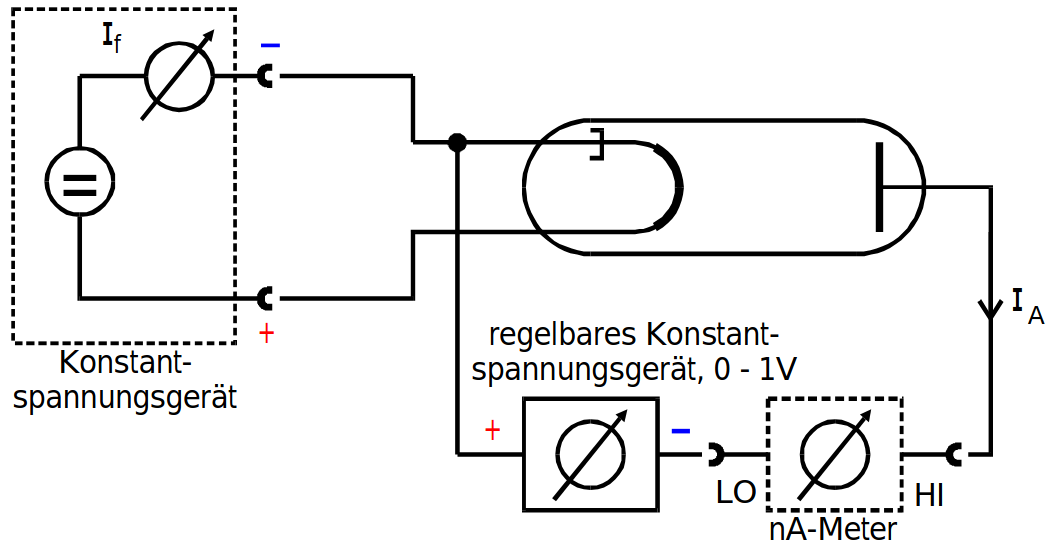
\includegraphics[width=\textwidth]{content/data/aufbau.png}
    \caption{Der Aufbau welcher zur Messung des Anlaustroms genutzt wird. Die Abbildung wurde aus \cite[10]{anleitung} entnommen.}
    \label{fig:aufbau}
\end{figure}
Da die zu messenden Ströme sehr gering sind, wird zur Messung ein sehr kurzes Kabel genutzt.
Zudem sollte während der Messung das Kabel zwischen Anode und Messgerät nicht berührt werden, da schon die leichte elektrische Ladung der Haut die Messung beeinflusst.
Die Diode ist wie zuvor an ein konstant Spannungsgerät angeschlossen, welches den Heizstrom an der Kathode erzeugt.
Zwischen Anode und Kathode wird eine Spannungsquelle angeschlossen.
Diese erzeugt eine Bremsspannung, im Bereich von $0 - 1 \SI{}{\V}$, zwischen Kathode und Anode.
Zur Messung wird nun der Heizstrom an der Kathode auf $\SI{2.5}{\A}$ gebracht.
Nun wird bei einer Bremsspannung von $\SI{0}{\V}$ die Messung gestartet und der Wert notiert, den das nano-Ampere Meter anzeigt.
Die Spannung wird jetzt um $\SI{0.1}{\V}$ erhöht und der Strom zwischen Anode und Kathode wird erneut notiert.
Die Messung wird bis zu einer Spannung von $\SI{1}{\A}$ weitergeführt.